%http://www.bakoma-tex.com/doc/latex/tikz-3dplot/tikz-3dplot_documentation.pdf
\tdplotsetmaincoords{70}{110}
\begin{tikzpicture}[tdplot_main_coords]
\draw[thick,->] (0,0,0) -- (1,0,0) node[anchor=north east]{$x$};
\draw[thick,->] (0,0,0) -- (0,1,0) node[anchor=north west]{$y$};
\draw[thick,->] (0,0,0) -- (0,0,1) node[anchor=south]{$z$};
\tdplotsetrotatedcoords{60}{40}{30}
\draw[thick,color=blue,tdplot_rotated_coords,->] (0,0,0) --
(.7,0,0) node[anchor=north]{$x$};
\draw[thick,color=blue,tdplot_rotated_coords,->] (0,0,0) --
(0,.7,0) node[anchor=west]{$y$};
\draw[thick,color=blue,tdplot_rotated_coords,->] (0,0,0) --
(0,0,.7) node[anchor=south]{$z$};
\end{tikzpicture}

\begin{tikzpicture}[isometric view]
% top half
\draw[ball color=gray!50, opacity=1] {[canvas is xy plane at z=0] (135:2) arc (135:315:2)} arc (0:180:2cm);
% bottom half
\begin{scope}[yshift=-0cm]
%\draw[ball color=red!10,shading angle=180] (0,0) circle (2);
%\draw[ball color=gray!10] {[canvas is xy plane at z=0] (315:2) arc (315:135:2)} arc (180:360:2cm);
\end{scope}
\end{tikzpicture}

\usetikzlibrary{arrows.meta}

\definecolor{plum}{rgb}{0.36078, 0.20784, 0.4}
\definecolor{chameleon}{rgb}{0.30588, 0.60392, 0.023529}
\definecolor{cornflower}{rgb}{0.12549, 0.29020, 0.52941}
\definecolor{scarlet}{rgb}{0.8, 0, 0}
\definecolor{brick}{rgb}{0.64314, 0, 0}
\definecolor{sunrise}{rgb}{0.80784, 0.36078, 0}
\definecolor{lightblue}{rgb}{0.15,0.35,0.75}
\definecolor{carolina}{RGB}{153, 186, 221}

% A custom arrowhead for use on x, y, z axes
\tikzstyle{axisarrow} = [-{Latex[inset=0pt,length=5pt]}]
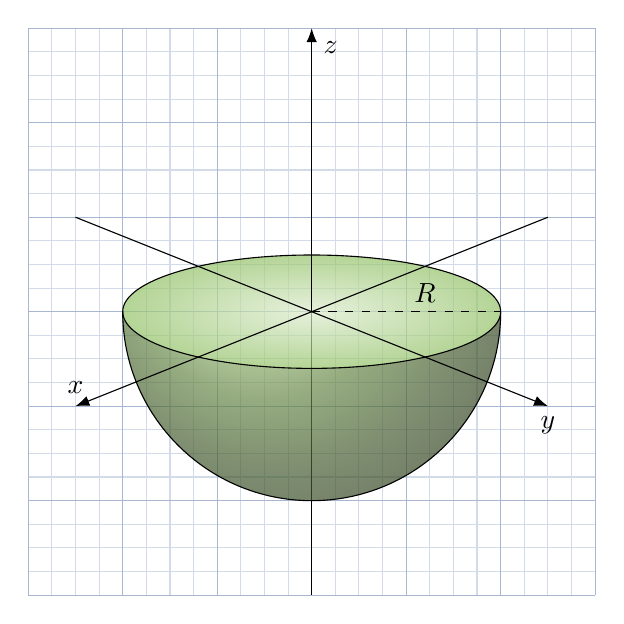
\begin{tikzpicture}[scale=1.2]
    % Draw the background grid.
    \draw [cornflower!20,step=0.25,thin] (-3,-3) grid (3,3);
    \draw [cornflower!40,step=1.0,thin] (-3,-3) grid (3,3);

    
    % The obscured part of the z-axis
    \draw (0,0) -- (0,-3);

    % Draw a shaded ball, but clip so only the lower half shows.
    % The arc in the clipping region is the foreground part of the equator
    \begin{scope}
        \clip(-3,-3) -- (-3,0) -- (-2,0) arc (180:360:2cm and 0.6cm) -- (3,0) -- (3,-3) -- (-3,-3);
        \shade[ball color=chameleon!60!white, opacity=0.70] (0,0) circle (2cm);
    \end{scope}

    % Draw the disc on top of the hemisphere.
    \shade[shading=radial, inner color=chameleon!20!white, outer color=chameleon!60!white, opacity=0.70] (2,0) arc (0:360:2cm and 0.6cm); 
    
    % Outline the disk in black
    \draw (2,0) arc (0:360:2cm and 0.6cm);

    % Outline the hemisphere in black
    \draw (-2,0) arc (180:360:2cm and 2cm);

    % A dashed line and label indicating the radius
    \draw [dashed] (0,0)--(2,0);
    \node at (1.2,.2) {$R$};

    % The rest of the z-axis
    \draw[axisarrow] (0,0) -- (0,3);
    \node at (.2,2.8) {$z$};

    % The y-axis
    \draw[axisarrow] (-2.5,1) -- (2.5,-1);
    \node at (2.5,-1.2) {$y$};

    % The x-axis
    \draw[axisarrow] (2.5,1) -- (-2.5,-1);
    \node at (-2.5,-0.8) {$x$};

\end{tikzpicture}

%https://latex.org/forum/viewtopic.php?t=25316
\tikzstyle{axisarrow} = [-{Latex[inset=0pt,length=5pt]}]
\tdplotsetmaincoords{70}{110}
\pgfmathsetmacro{\rvec}{1.2}
%\pgfmathsetmacro{\thetavecc}{55}
%\pgfmathsetmacro{\phivecc}{35}
%\pgfmathsetmacro{\thetaveccc}{39.7}
%\pgfmathsetmacro{\phiveccc}{55}
\begin{tikzpicture}[scale=3,tdplot_main_coords]
\shadedraw[tdplot_screen_coords,ball color = white] (0,0) circle (\rvec);
%-----------------------
%\coordinate (O) at (0,0,0);
%\tdplotsetcoord{B}{\rvec}{\thetavecc}{\phivecc}
%\tdplotsetcoord{C}{\rvec}{\thetaveccc}{\phiveccc}

% main coordinate axes
\draw[thick,->] (0,0,0) -- (1.7,0,0) node[anchor=north east]{$x$};
%\draw[thick,->] (0,0,0) -- (0,1.7,0) node[anchor=north west]{$y$};
\draw[thick,->] (0,0,0) -- (0,0,1.7) node[anchor=south]{$z$};

%\draw[-stealth,very thick,color=blue] (O) -- (B);
%
%\draw[-stealth,very thick,color=green!60!black] (O) -- (C);
%\draw[dashed, color=blue] (O) -- (Bxy);
%\draw[dashed, color=blue] (B) -- (Bxy);
%\draw[dashed, color=green!60!black] (O) -- (Cxy);
%\draw[dashed, color=green!60!black] (C) -- (Cxy);

%\tdplotdrawarc[color=blue]{(O)}{0.3}{0}{\phivecc}{anchor=north}{$\lambda_A$}

%\tdplotsetthetaplanecoords{\phivecc}

%\tdplotdrawarc[color=blue,tdplot_rotated_coords]{(0,0,0)}{0.3}{90}{\thetavecc}{anchor=south west}{$\varphi_A$}

%\tdplotdrawarc[color=green!40!black]{(O)}{0.7}{0}{\phiveccc}{anchor=north}{$\lambda_B$}

%\tdplotsetthetaplanecoords{\phiveccc}

%\tdplotdrawarc[color=green!40!black,tdplot_rotated_coords]{(0,0,0)}{0.7}{90}{\thetaveccc}{anchor=south west}{$\varphi_B$}

%\draw[dashed] (\rvec,0,0) arc (0:360:\rvec);
%\draw[thick] (\rvec,0,0) arc (0:110:\rvec);
%\draw[thick] (\rvec,0,0) arc (0:-70:\rvec);

%\tdplotsetthetaplanecoords{40}

\draw[axisarrow,color=blue] (0,0,0) -- (0,\rvec,0) node[anchor=north west]
{$\vec{y}_1$};
\draw[dashed, color=blue] (0,0,0) -- (0,\rvec + 0.5,0) node[anchor=north west] 
{};

\draw[axisarrow,color=green] (0,0,0) -- (0.5,0.5,0.707,0) node[anchor=north west]
{$\vec{y}_2$};

\tdplotsetrotatedcoords{45}{0}{45}
\draw[very thick,tdplot_rotated_coords] (\rvec,0,0) arc (360:294:\rvec);

\tdplotsetrotatedcoords{150}{50}{20}
\draw[thick,color=blue,tdplot_rotated_coords,->] (0,0,0) --
(\rvec,0,0) node[anchor=north]{$x$};
\draw[thick,color=blue,tdplot_rotated_coords,->] (0,0,0) --
(0,\rvec,0) node[anchor=west]{$y$};
\draw[thick,color=blue,tdplot_rotated_coords,->] (0,0,0) --
(0,0,\rvec) node[anchor=south]{$z$};

\draw[thick,tdplot_rotated_coords] (\rvec,0,0) arc (0:115:\rvec);
\draw[dashed,tdplot_rotated_coords] (\rvec,0,0) arc (0:360:\rvec);
\draw[thick,tdplot_rotated_coords] (\rvec,0,0) arc (360:294:\rvec);

%\tdplotsetthetaplanecoords{55}
%\draw[thick,tdplot_rotated_coords] (\rvec,0,0) arc (0:147:\rvec);
%\draw[very thick,color=red,tdplot_rotated_coords] (\rvec,0,0) arc (0:40:\rvec);
%\draw[dashed,tdplot_rotated_coords] (\rvec,0,0) arc (180:-40:-\rvec);
%\draw[thick,tdplot_rotated_coords] (\rvec,0,0) arc (360:334:\rvec);

%\tdplotsetrotatedcoords{-79.1}{-120}{27.3}
%\draw[very thick,color=red,tdplot_rotated_coords] (\rvec,0,0) arc (0:21:\rvec);
\end{tikzpicture}

%https://latex.org/forum/viewtopic.php?t=25316
\tdplotsetmaincoords{60}{110}
\pgfmathsetmacro{\rvec}{1.2}
\begin{tikzpicture}[scale=3,tdplot_main_coords]

\coordinate (O) at (0,0,0);

% main coordinate axes
\draw[thick,->] (0,0,0) -- (\rvec,0,0) node[anchor=north east]{$x$};
\draw[thick,->] (0,0,0) -- (0,\rvec,0) node[anchor=north west]{$y$};
\draw[thick,->] (0,0,0) -- (0,0,\rvec) node[anchor=south]{$z$};

% rotated axis
\tdplotsetrotatedcoords{150}{50}{20}
\draw[thick,color=blue,tdplot_rotated_coords,->] (0,0,0) --
(\rvec,0,0) node[anchor=north]{$x$};
\draw[thick,color=blue,tdplot_rotated_coords,->] (0,0,0) --
(0,\rvec,0) node[anchor=west]{$y$};
\draw[thick,color=blue,tdplot_rotated_coords,->] (0,0,0) --
(0,0,\rvec) node[anchor=south]{$z$};

\draw[thick,color=blue,tdplot_rotated_coords] (\rvec,0,0) arc (0:115:\rvec);
\draw[dashed,color=blue,tdplot_rotated_coords] (\rvec,0,0) arc (0:360:\rvec);
\draw[thick,color=blue,tdplot_rotated_coords] (\rvec,0,0) arc (360:294:\rvec);

\draw[tdplot_screen_coords,color=black, opacity=0.1,fill=gray] (0,0) 
 circle (\rvec);

\draw[thick,color=blue,tdplot_screen_coords] (\rvec,0,0) arc (0:144:\rvec);
\draw[thick,color=blue,tdplot_screen_coords] (\rvec,0,0) arc (360:323:\rvec);

\end{tikzpicture}

%\tdplotsetmaincoords{70}{110}
%\begin{tikzpicture}[scale=2,line join=bevel,tdplot_main_coords,fill opacity=1]
%    \tdplotsphericalsurfaceplot[parametricfill]{72}{36}{2}{green}{
%        120*floor(\tdplottheta/120)
%    }{}{}{}
%\end{tikzpicture}


\tdplotsetmaincoords{60}{110}
\pgfmathsetmacro{\radius}{1}
\pgfmathsetmacro{\thetavec}{0}
\pgfmathsetmacro{\phivec}{0}

\begin{tikzpicture}[scale=2,tdplot_main_coords]
%draw the main coordinate system axes
\draw[thick,->] (0,0,0) -- (0,0,1) node[anchor=south]{$z$};
\draw[thick,->] (0,0,0) -- (1,0,0) node[anchor=north west]{$x$};
\draw[thick,->] (0,0,0) -- (0,1,0) node[anchor=south]{$y$};

\tdplotsetthetaplanecoords{\phivec}
\draw[dashed,tdplot_rotated_coords] (\radius,0,0) arc (0:90:\radius);
\draw[dashed] (\radius,0,0) arc (0:360:\radius);
\shade[ball color=blue!10!white,opacity=0.2] (1cm,0) arc (0:-180:1cm and 5mm) arc (180:0:1cm and 1cm);
% (-z x y)
\end{tikzpicture}

\tdplotsetmaincoords{0}{0}
\tdplotsetrotatedcoords{0}{0}{0}
\begin{tikzpicture}[tdplot_main_coords]
\begin{scope}
    \clip (-1.5,0) rectangle (1.5,1.5);
    \draw (0,0) circle(1.5);
    \draw (-1.5,0)  rectangle(1.5,0);
\end{scope}
\end{tikzpicture}

%https://tex.stackexchange.com/questions/368604/how-to-draw-a-half-and-half-colored-circle
\pgfmathsetmacro{\radius}{2}
\begin{tikzpicture}
    \draw[thick,->] (0,0,0) -- (\radius,0,0) node[anchor=north west]{$\vec{\lambda}_1$};
    \draw[thick,->] (0,0,0) -- (-0.684, 1.879,0) node[anchor=south east]{$\vec{\lambda}_2$};    
    \fill[red,opacity=0.2] (0,0) circle (\radius); % Fill circle with base colour (arg#2)
    \fill[blue, opacity=0.2] (0,0) -- (135:\radius) arc (135:315:\radius) -- cycle; % Fill a half circle filled with second colour (arg#1), if specified
\end{tikzpicture}

\tdplotsetmaincoords{40}{0}
\tdplotsetrotatedcoords{150}{50}{20}
\begin{tikzpicture}[scale=2,line join=bevel,tdplot_rotated_coords,fill opacity=1]
\pgfsetlinewidth{.0pt}
    \tdplotsphericalsurfaceplot[parametricfill]{72}{36}{2}{transparent!0}{
        180*floor(\tdplotphi/180)
    }{}{}{}
\end{tikzpicture}

\afterpage{
    \clearpage
    \thispagestyle{empty}
    \begin{landscape}
        \topskip0pt
        %\vspace*{\fill}
        \begin{table}[htb!]
        \centering 
        %\tiny
        \begin{tabular}{ccccccccccccccccc}
            \toprule
            Resource    & \multicolumn{4}{c}{100 shots} 
                        & \multicolumn{4}{c}{100 shots} 
                        & \multicolumn{4}{c}{100 shots} 
                        & \multicolumn{4}{c}{500 shots}\\
            \midrule
            {}  & 00 & 01 & 10 & 11 
                & 00 & 01 & 10 & 11 
                & 00 & 01 & 10 & 11 
                & 00 & 01 & 10 & 11\\
            Aer Simulator   & 17.5 & 19.1 & 17.5 & 19.1 
                            & 17.5 & 19.1 & 17.5 & 19.1 
                            & 17.5 & 19.1 & 17.5 & 19.1 
                            & 17.5 & 19.1 & 17.5 & 19.1\\
            Nairobi         & 17.5 & 19.1 & 17.5 & 19.1 
                            & 17.5 & 19.1 & 17.5 & 19.1 
                            & 17.5 & 19.1 & 17.5 & 19.1 
                            & 17.5 & 19.1 & 17.5 & 19.1\\               
            Perth           & 17.5 & 19.1 & 17.5 & 19.1 
                            & 17.5 & 19.1 & 17.5 & 19.1 
                            & 17.5 & 19.1 & 17.5 & 19.1 
                            & 17.5 & 19.1 & 17.5 & 19.1\\
            Oslo            & 17.5 & 19.1 & 17.5 & 19.1 
                            & 17.5 & 19.1 & 17.5 & 19.1 
                            & 17.5 & 19.1 & 17.5 & 19.1 
                            & 17.5 & 19.1 & 17.5 & 19.1\\
            Jakarta         & 17.5 & 19.1 & 17.5 & 19.1 
                            & 17.5 & 19.1 & 17.5 & 19.1 
                            & 17.5 & 19.1 & 17.5 & 19.1 
                            & 17.5 & 19.1 & 17.5 & 19.1\\   
            Lagos           & 17.5 & 19.1 & 17.5 & 19.1 
                            & 17.5 & 19.1 & 17.5 & 19.1 
                            & 17.5 & 19.1 & 17.5 & 19.1 
                            & 17.5 & 19.1 & 17.5 & 19.1\\                            
            \bottomrule        
        \end{tabular}
        \captionof{table}{Example of probability distributions for circuit's classical measurement outcomes $\{00, 01, 10, 11\}$ obtained with different IBM Quantum systems and simulators. The prepare-and-measure scenario is that with state $\ket{\Psi}=\frac{3 + i \sqrt{3}}{4} \ket{0} - \frac{1}{2} \ket{1}$ and POVM measure $\mathbb{P}_4 = \{\frac{1}{2}\ket{0}\bra{0}, \frac{1}{2}\ket{1}\bra{1}, \frac{1}{2}\ket{+}\bra{+}, \frac{1}{2}\ket{-}\bra{-} \}$.}
        \label{table:quantum_results}
        \end{table}
    \end{landscape}
    \clearpage
}
